\subsection{Monitoraggio e Valutazione}
Quando vedete una freccia circolare bisogna pensare al \textbf{PDCA} (Plan Do
Check Act). Infatti, ormai tutti i progetti sono circolari. \emph{Kaizen} è
una parola giapponese che vuol dire “miglioramento continuo”. Quando si vede
che c’è un delta, ovvero uno scostamento tra valore atteso e valore ottenuto,
si cerca di operare per migliorarlo. Una volta raggiunti gli obiettivi
prefissati, come previsto dal \textbf{PDCA}, bisogna fissare dei nuovi
obiettivi da raggiungere per migliorarsi continuamente.

\begin{itemize}
\item ME1: monitorare e valutare le prestazioni dell'IT;
\item ME2: monitorare e valutare i controlli interni;
\item ME3: assicurare la conformità a leggi e normative esterne;
\item ME4: istituire l'IT governance.
\end{itemize}

Sulla nuova normativa di privacy se l'azienda non intraprenderà le procedure
adeguate per preservare la privacy, avrà delle multe fino al 5\% del fatturato
e la possibilità di andare a processo.






\section{CMM}

Il \textit{Capability Maturity Model} (CMM) è nato come modello per
valutare la maturità della capacità
di sviluppo del Software. Ora questa categorizzazione viene utilizzata
anche per valutare la maturità di un'azienda.
In particolare nel COBIT questo modello trova impiego per valutare la
capacità di governare i processi di gestione dell'IT.
I vari livelli del CMM sono riportati nella Figura~\ref{fig:cmm:levels}.

In generale gli investitori saranno più portati a investire in aziende che
hanno un CMM alto rispetto ad uno basso.
I livelli bassi, dal livello 2 in giù, sono legati fortemente all'abilità
dei singoli.
I livelli alti sono caratterizzati
dalla documentazione dei processi (Lv. 3),
dalle metriche (Lv. 4) e dal miglioramento continuo (Lv. 5).
Inoltre dal Livello 4 in su,
l'automatizzazione dei processi di controllo permette un risparmio sul
TCO (Total Cost of Ownership).

Il CMM è stato superato dal CMMI \textit{Capability Maturity Model Integration}.




\begin{figure}[h!]
        \begin{center}
                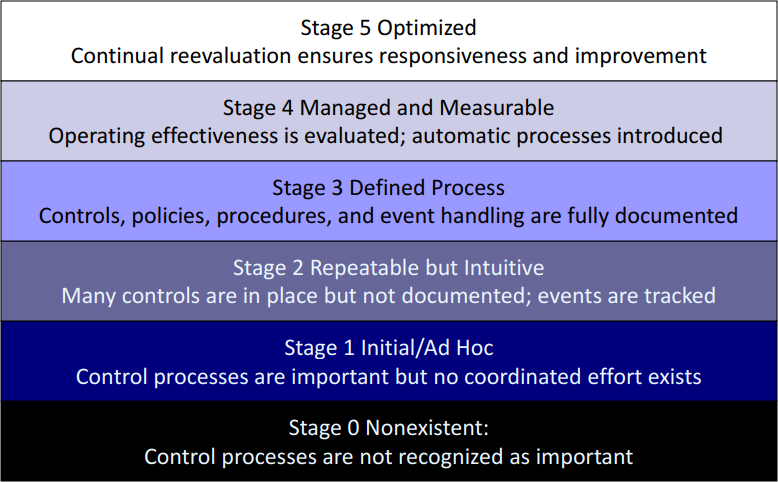
\includegraphics[scale=2.0]{res/img/maturity_level}
        \end{center}
        \caption{I 5 livelli del Capability Maturity Model (CMM).}
        \label{fig:cmm:levels}
\end{figure}




\subsection{Livello 0 - Non esistente}

Vi è una totale assenza
di processi gestionali dell'IT.

\subsection{Livello 1 - Initial - Esecuzione informale}

La progettazione della sicurezza è definita in maniera povera, i problemi di
sicurezza sono trattati in maniera reattiva: si reagisce
alla minaccia, portando prima o poi l'attacco a vincere. Non ci sono piani di
contingenza\footnote{I piani di contingenza sono dei piani che dettano le
azioni da compiere in caso si verificano delle situazioni d'emergenza.}. I
budget, la qualità, le funzionalità e i progetti vengono schedulati \textit{ad
hoc}. Non è in atto alcun tipo di
pianificazione e i processi sono ad hoc e disorganizzati.

\subsection{Livello 2 - Managed - Pianificato e Tracciato}

Le procedure vengono definite a livello di progetto. La definizione,
pianificazione e le performance diventano de-facto standard da progetto a
progetto. Gli eventi vengono tracciati Le funzionalità comuni includono:
pianificazione, disciplina, verifica e tracciamento delle performance.
Si ha ancora un approccio di tipo reattivo agli
eventi che accadono, ma si comincia ad definire processi ed ad avere
pianificazioni per i progetti;


\subsection{Livello 3 - Ben definito}


Si cominciano a definire processi anche per
l'organizzazione in toto e si comincia ad avere un approccio 
proattivo ai  problemi e si \textbf{documentano} i processi.

I processi di sicurezza sono standardizzati all'interno dell'organizzazione e
il personale viene addestrato per assicurarsi che abbia le conoscenze e le
skill necessarie. In aggiunta, le misure vengono basate su un processo
definito e gli audit tracciano le performance. Le funzionalità più comuni
includono: definire un processo standard, eseguire il processo definito e
coordinare le pratiche relative alla sicurezza.

\subsubsection{Policy, procedure e standard}

\paragraph*{Obiettivo di una policy:} descrive \textit{cosa} deve essere
soddisfatto.

\paragraph*{Controllo della policy:} tecniche per raggiungere l'obiettivo,
suddivise in
\begin{itemize}
  \item \textbf{Procedure:} definiscono come la policy deve essere perseguita;
  \item \textbf{Standard:} regola, metrica o vincolo specifico che implementa
  la policy.
\end{itemize}

La definizione di policy, procedura, standard e linee guida vengono
riportate nella Figura~\ref{fig:doc:policy}.


\begin{figure}[h!]
        \begin{center}
                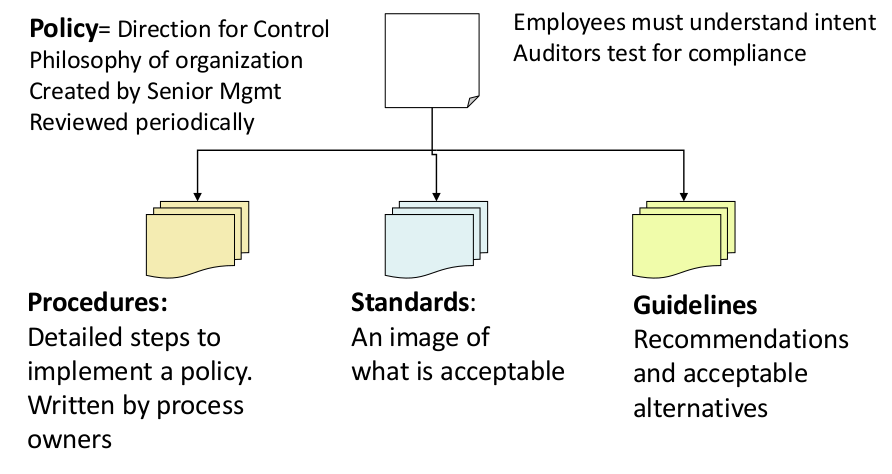
\includegraphics[scale=0.4]{res/img/documentation_policy}
        \end{center}
        \caption{Definizione di policy, procedura, standard e linee
        guida e la loro relazione.}
        \label{fig:doc:policy}
\end{figure}

\paragraph*{Esempi di policy}

I \textbf{rischi} dovrebbero essere gestiti utilizzando dei controlli e delle
contromisure appropriate per raggiungere dei livelli accettabili a dei costi
accettabili. Il \textbf{monitoraggio} e le \textbf{metriche} dovrebbero essere
implementate, gestite e mantenute per fornire una certezza continua che tutte
le policy sulla sicurezza siano rispettate e i controlli oggettivi siano
riscontrati. Le \textbf{capacità di risposta ad incidenti} sono implementate e
gestite sufficientemente per garantire che gli incidenti non affliggano
materialmente la capacità dell'organizzazione di continuare le proprie
operazioni.
La \textbf{business continuity} e il \textbf{recovery plan} dovrebbero essere
sviluppati, manutenuti e testati in modo da assicurare la capacità
dell'organizzazione di proseguire con le proprie attività sotto tutte le
condizioni.


Nota: una cattiva \textit{policy} fa riferimento alla tecnologia. Le
\textit{policy} dettano la filosofia dell'azienda.



\subsubsection{Definizioni della qualità}

\paragraph*{Quality assurance:} assicurarsi che tutto lo staff stia seguendo i
processi della qualità definiti.

\paragraph*{Controllo della qualità:} condurre test per validare che il
software è privo di difetti e corrisponde alle aspettative dell'utente.

\subsection{Livello 4 - Quantitatevely Managed - Metriche}

Esistono degli obiettivi misurabili per la qualità della sicurezza, le misure
sono correlate agli obiettivi del business dell'organizzazione. Le
funzionalità comuni includono: stabilire degli obiettivi misurabili di qualità
e una gestione oggettiva delle performance (SLA).
È tutto scritto e documentato: sono presenti politiche, procedure, standard e 7
linee guida.

\subsubsection{Metriche}

Le metriche permettono ad auditor differenti di attestare che i programmi per
la sicurezza vengono attuati. Monitorare il raggiungimento di controlli
oggettivi è più importante che perfezionare le procedure di sicurezza.

Senza metriche quantitative si lascia spazio alla soggettività.

\begin{figure}[h!]
        \begin{center}
                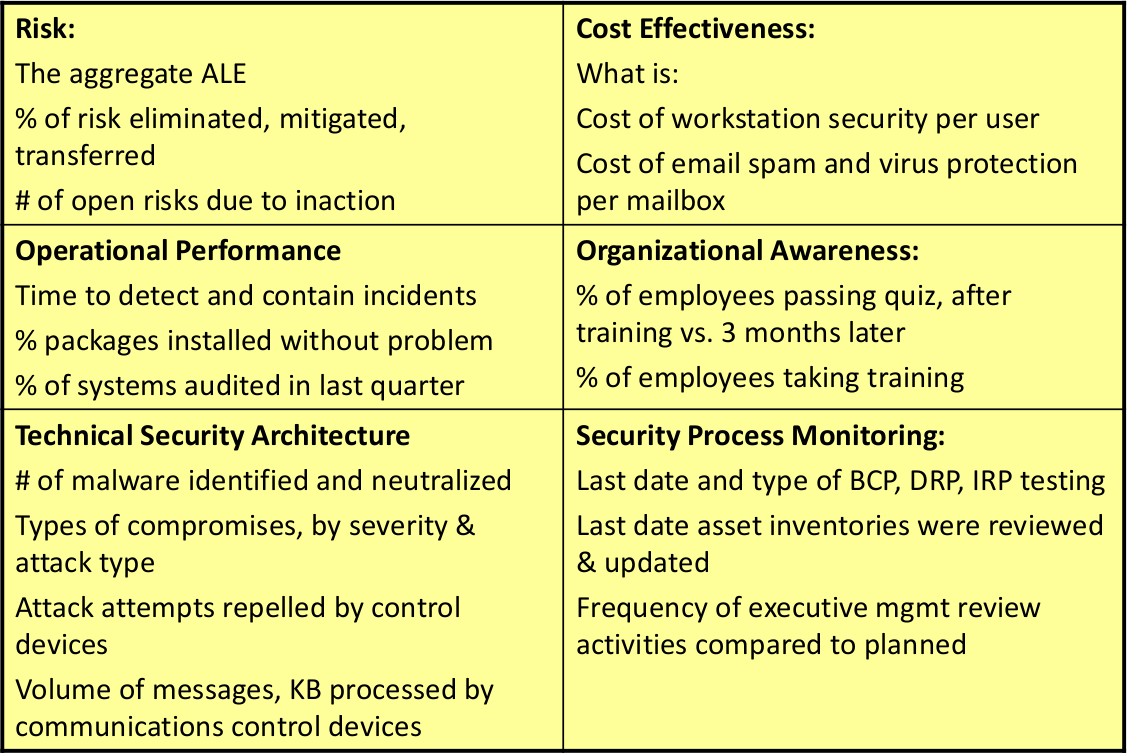
\includegraphics[scale=1.5]{res/img/metriche}
        \end{center}
        \caption{Esempi di metriche per un'azienda.}
\end{figure}

\paragraph*{Metriche operazionali}

Le metriche di tipo operazionale includono metriche su come eseguire
un corretto \textit{patching} dei sistemi.

Confrontare le metriche con quelle di altre aziende permette di capire quanto
siamo un possibile \textit{target} per gli attaccanti.

\paragraph*{Metriche di tipo strategico}

Sono i piani legati al rischio, come il \textit{disaster recovery}.
Il rapporto di audit è una metrica importantissima perché fa capire come
lavorano l'azienda e l'auditor.

\paragraph*{Compliance interna}

La conformità (\textit{compliance}) assicura la conformità con le policy
organizzative. Compliance e errore interno sono dati importanti perché
fanno capire all'azienda quanto è allineata con gli obiettivi strategici che
si è prefissata.


\subsection{Livello 5 - Optimized - Miglioramento continuo}

Una volta che è in atto il \textbf{miglioramento continuo}
dei processi che vengono a loro volta misurati tramite metriche l'azienda
può puntare ad ottimizzarli il più possibile.
  
Il miglioramento continuo parte dalle misure e dagli eventi sulla sicurezza.
Vengono valutate nuove tecnologie e nuovi processi. Le funzionalità comuni
includono: miglioramento delle capacità organizzative e dell'efficacia dei
processi (ROI).

Prima avere un cambio tecnologico di fondo era raro, oggi avviene ogni 3 anni.
Chi prende la tecnologia e la incorpora si prende la fetta di mercato.

Le grandi società fanno \textit{scouting} di nuove tecnologie. Il vantaggio di
essere un'azienda piccola è che si può essere aggressivi e investire, aiutando
il movimento economico. Questo ci dice che aziende come Google non ci
saranno per sempre. Non si è ancora capito a dove possa portare il cambiamento
tecnologico. Un'altra area importante è l'intelligenza artificiale legata
alla sicurezza.

\subsection{Relazione tra gli standard di sicurezza}

ISO 27001 e il COBIT sono gli standard di sicurezza di base. La \textit{gap
analysis} (differenza tra dove vorremmo essere e dove siamo) ci aiuta a capire
dove sono presenti le lacune da colmare.

\begin{figure}[h!]
        \begin{center}
                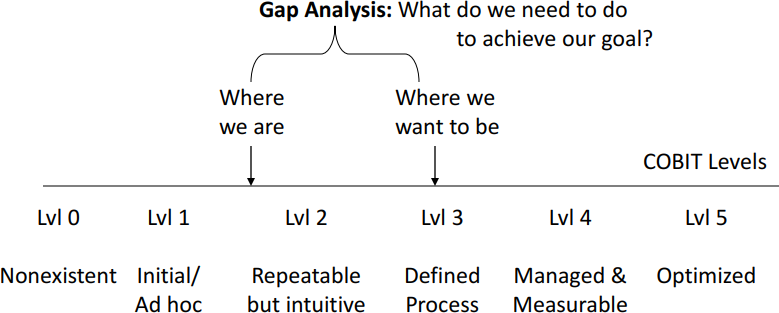
\includegraphics[scale=2.0]{res/img/security_standard}
        \end{center}
        \caption{I 5 livelli del Capability Maturity Model (CMM) e il
        loro rapporto con un programma di sicurezza.}
\end{figure}


\subsubsection{Esercizi}

Gli esercizi sono disponibili in \ref{esSM:COBIT}

\chapter{Policy and Governance}
\label{PG}

\section{Governance}

\textbf{Corporate governance:} è la leadership da parte dei direttori
aziendali nel creare e presentare il valore agli stakeholders.\\
\newline
\textbf{IT governance:} si assicura del corretto allineamento dell'IT con gli
obiettivi aziendali.



\section{Strategic Planning Process}
\label{PG:SPP}

Oggi come oggi una \textbf{pianificazione strategica} nell'IT è in 3 anni, in
quanto tra 5 anni nessuno sa cosa ci sarà. Quindi la lunghezza dei piani si è
accorciata, specialmente nel settore informatico in quanto la pressione
tecnologica è altissima. Questa pianificazione è destinata ad accorciarsi
grazie all'intelligenza artificiale, che aiuterà gli umani a prendere
decisioni. La \textbf{pianificazione tattica} dura un anno e permette
all'organizzazione di muoversi verso gli obiettivi strategici, mentre la
\textbf{pianificazione operazionale} definisce piani dettagliati o tecnici.

\begin{figure}[H]
        \begin{center}
                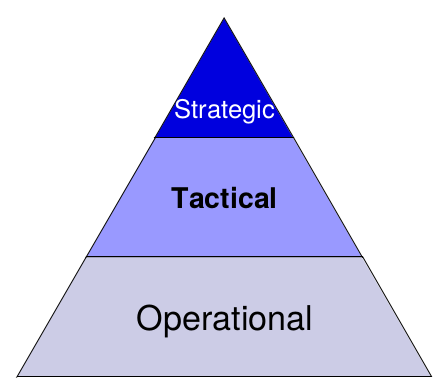
\includegraphics[scale=0.4]{res/img/planning_process}
        \end{center}
        \caption{Piramide dei differenti tipi di pianificazione.}
\end{figure}

